\documentclass[a4paper,12pt]{report}
\usepackage{hyperref}
\usepackage{fancyhdr}
\hypersetup{colorlinks,unicode, pdfborder=0 0 0}
\usepackage{amsfonts}
\usepackage{amssymb}
\usepackage[T1]{fontenc}
\usepackage[utf8]{inputenc}
\PassOptionsToPackage{defaults=hu-min}{magyar.ldf}
\usepackage[magyar]{babel}
\setcounter{secnumdepth}{5}
\usepackage{graphicx}

\newcommand{\PK}[1]{\textbf{#1}}
\newcommand{\FK}[1]{\underline{#1}}
\newcommand{\TABLA}[1]{\noindent\MakeUppercase{#1}}
\newcommand{\TMEZO}[2]{\MakeUppercase{#1}.{\underline{#2}}}


%opening
\title{%
    \Huge \textbf{Mérőeszköz kalibrálás \\ és nyilvántartó rendszer} \\
    \vspace*{72pt}
    \textbf{Rendszerterv}
    }

\author{Szikora György}
\date{2020}

\pagestyle{fancy}
\fancyhead[L]{}
\fancyhead[C]{}
\fancyhead[R]{\scriptsize{\rightmark}}
\fancyfoot[L]{\footnotesize{Szikora György}}
\fancyfoot[C]{\thepage}
\fancyfoot[R]{}
\renewcommand{\headrulewidth}{0.4pt}
\renewcommand{\footrulewidth}{0.4pt}

\begin{document}

\maketitle

\tableofcontents
\listoffigures
\listoftables

\part{Bevezetés}
\chapter{A tervezett rendszer}
A BKV Vasúti Járműjavító Kft. 9001:2015-ös ISO rendszerben végzi 
tevékenységeinek jelentős részét. A minőségbiztosítás fontos eleme a mérő-, 
ellenőrző- és vizsgáló eszközök, berendezések nyilvántartása, megfelelő 
működésük rendszeres ellenőrzése, a napi karbantartáson túlmutató ápolása, 
esetleges javítása, a mért értékek helyességének biztosításának érdekében, 
végzett kalibrálás, egyes esetekben a hitelesítés.

A Kft. az 90-es évek végétől a mérő-, ellenőrző-, vizsgáló eszközök 
nyilvántartására egy mára elavultnak tekinthető programot használ, ami nem,
vagy alig biztosítja az elégséges feltételeket az idő közben életbe lépet 
\textit{24/2016 (VII. 18.) NFM rendelet} követelményeinek betartására. Arról 
született döntés, hogy a felhasználó igények és a megfelelés érdekében egy új 
rendszert kell megtervezni, majd bevezetni.

Az új rendszer tervezésekor figyelembe kell venni:
\begin{itemize}
\item a régi rendszerből átvehető adatokat, azok helyességét,
\item a régi rendszer használható funkciónak bevezethetőségét,
\item a felhasználói igényeket,
\item a vonatkozó, jelenleg hatályos jogszabályi és más követelményeket,
\item az új rendszer ne kötődjön egyetlen számítógéphez,
\item a rendszer adatai legyen kellően védettek,
\item az új rendszer üzembe állításához szükséges infrastrukturális és szoftver 
környezetet.
\end{itemize}

\chapter{A jelenlegi rendszer}
\section{A jelenlegi rendszer bemutatása}
A jelenleg használt mérőeszköz és azok kalibrálási állapotát tartalmazó rendszer 
egy mára már elavult Clipper, vagy dBase alkalmazás. Erre utalnak a Kft.
hálózati meghajtóján tárolt fájlok \textit{DBF}, illetve \textit{NTX} 
kiterjesztése.

A hálózatos kialakítás előnye, hogy elvileg minden olyan eszközről elérhető az
adatbázis, amely a keretprogramon keresztül képes csatlakozni hozzá. Egyúttal 
kockázatot is jelent, hogy a hálózati meghajtón lévő fájlok egy alacsony szintű 
hozzáférés esetén is könnyen megváltoztathatók, tekintettel arra, hogy a dBase 
adatfájlok strukturált szerkezete szövegszerkesztő, táblázatkezelő 
alkalmazással egyszerűen módosíthatók.

A DBF fájlok tanulmányozása az alábbiakat tárta fel:
\begin{itemize}
\item az első bejegyzések 1999-ben keletkeztek,
\item az adatbázis inkonzisztenciájára utaló jelek láthatók(!) ,
\item egyes mezők kitöltése esetleges, nem következetes,
\item az adatok egy része meglévő Kft.-s nyilvántartásokra épül, például a
dolgozók azonosítása,
\item másrészt nem „SAP kompatibilis”, a SAP 2001-ben került bevezetésre, emiatt 
az egyik rendszerből kinyert adat direkt módon nem használható fel a másik 
rendszerben.
\end{itemize}
A keretprogram tanulmányozása rámutatott, hogy:
\begin{itemize}
\item a rendszerből releváns riportok kinyerésére csak képernyőkép útján van
lehetőség,
\item nincs mód az aktív-inaktív állapotok rögzítésére,
\item az adattáblák kulcs és leíró mezői keverednek.
\item az egyik fő hiba, hogy a jelenlegi ,,adatbázis'' inkonzisztens.
\end{itemize}

\section{A jelenlegi rendszer további használatának lehetősége}

A jelenlegi rendszer javítására nincs mód, az eredeti forráskód nincs meg, csak
a futtatható állománnyal rendelkezik a Kft. 
A karaktergrafikus alkalmazás egyébként a feladat elvégzéshez tökéletes lenne, 
azonban a fejlesztői környezetet meg kellene vásárolni, illetve licence díjat 
kell fizetni érte.
Nem elegendő a jelenlegi adatbázis átültetése egy másik adatbázis motorra, mert
az eredeti adatbázis olyan tervezési hibákat tartalmaz, amit ki kell javítani, 
különben az új adatbázis működésében komoly zavart okoznak.

A jelenlegi rendszer a működés folyamatosságának érdekében tovább használható, 
de egyidejűleg el kell kezdeni a kialakítandó rendszer tervezését, a folyamatok 
feltárását, rögzítését.

A további inkonzisztencia növekedésének lassítása érdekében:
\begin{itemize}
\item lehetőleg kerülni kell új mérőeszköz típusok rögzítését,
\item  szöveges mezők kitöltésénél törekedni kell az azonos értékek azonos módon
történő rögzítésére,
\item az azonosító szerepű mezők kitöltése előtt ellenőrizni kell, hogy az 
azonosító létezik-e.
\end{itemize}

A jelenlegi rendszer adatai részben felhasználhatók az új rendszerben is, 
illetve a jelenlegi sémát kiindulásként fel lehet használni az új rendszer 
tervezéséhez.

\section{A régi rendszer hibái, az újratervezés szükségessége}

\subsection{Kulcsok hiánya}
A relációs adatbázisok az \textit{egyed - tulajdonság - kapcsolat} hármasra
épülnek. \textit{Egyed}nek nevezzük az adatokat tartalmazó táblákat, melyek 
sorai az \textit{egyed} előfordulások, a táblák oszlopai a 
\textit{tulajdonságok}, amelyek az egyed jellemzőit tárolják. A táblák 
közötti összefüggéseket, viszonyokat a táblák közötti \textit{kapcsolat} írja 
le.

Azokat a tulajdonságot, vagy tulajdonságokat, amelyek egyértelműen azonosítanak
egy-egy egyed előfordulást \textit{kulcs}nak nevezzük. Ha \textit{kulcs} egy 
elemű akkor egyszerű, ha több elemű akkor \textit{összetett kulcs}nak nevezzük.

A táblák közötti kapcsolatokat a \textit{kulcs}ok biztosítják. Ehhez az egyik 
tábla kulcsát egy másik táblának tartalmaznia kell és \textit{idegen-, vagy 
külső kulcs}nak nevezzük. Emellett fel kell állítani a szabályt aminek 
teljesülését az \textit{adatbázis motor} minden esetben automatikusan ellenőriz. 
Amennyiben a felállított szabály sérülne, úgy a motor nem engedi végrehajtani a 
kért műveletet.

A jelenlegi rendszerben, ha vannak is kulcsok, valószínűleg a szabályok leírása 
elmaradt, és semmi nem akadályozza meg, hogy a helytelen érték kerüljön a 
rendszerbe. Például a kalibrálást végezte oszlopban az érték hol 
\texttt{HARANGOZO}, hol \texttt{HRANGOZO}, de van \texttt{HARANGÓZO} és 
\texttt{HARANGÓZÓ} is.

\subsection{Kulcsok és szabályok hiánya, annak következményei}
A relációs adatbázisok táblái között a kulcsok írják le a kapcsolatot. Azzal, 
hogy az egyik tábla elsődleges kulcsát egy másik tábla idegen kulcsként 
tartalmazza, valamint a kulcsok között felállításra került a szabály, a táblák 
között kialkult a kapcsolat. Megfordítva, két tábla akkor van egymással 
kapcsolatban, ha az egyik tábla tartalmazza a másik tábla kulcsát.

Az összekapcsolás hiánya oda vezethet, hogy
\begin{itemize}
\item a felhasználó programnak kell ellenőrznie a kulcs szabályait,
\item ugyan ennek a programnak a feladata a szabály sérülésének kezelése,
\item ha a fentiek nem teljesünek, az adatbázis inkonzisztensé válhat.
\end{itemize}

Az inkonzisztencia veszélye abban nyilvánul meg, hogy lesznek olyan sorok az 
egyik táblában, amelyhez nem tartozik sor egy másik, a táblával kapcsolatban 
álló táblában.

A \ref{dolg} és \ref{kalib} táblák között a \textbf{dolgozókód} mező teremt
kapcsolatot. A DOLGOZÓ táblában ez a mező \textbf{kulcs}, míg a KALIBRÁLÁS 
táblában \textbf{idegen kulcs} szerepet tölt be.

\begin{figure}[ht!] \centering
\begin{tabular}{|l|l|}
        \hline
        \multicolumn{2}{|c|}{\textbf{DOLGOZÓ}}\\
        \hline
        \textbf{dolgozókód}&\textbf{dolgozónév}\\
        \hline
        HARANGOZO&Harangozó István\\
        \hline
        KOVACS&Kovács József\\
        \hline
        \dots&\dots\\
        \end{tabular}
        \caption{Példa DOLGOZÓ tábla}\label{dolg}
\end{figure}

\begin{figure}[ht!]\centering

\begin{tabular}{|r|c|l|}
        \hline
        \multicolumn{3}{|c|}{\textbf{KALIBRÁLÁS}}\\
        \hline
        \textbf{sorszám}&\textbf{...}&\textbf{dolgozókód}\\
        \hline
        1&\dots&HARANGOZO\\
        \hline
        2&\dots&HARANGOZO\\
        \hline
        \dots&\dots&\dots\\
        \hline
        104&\dots&KOVACS\\
        \hline
        \dots&\dots&\dots\\
\end{tabular}
\caption{Példa KALIBRÁLÁS tábla}\label{kalib}
\end{figure}
        

Ha a kulcsok közötti szabályok betartását a motor ellenőrzi, akkor a KALIBRÁLÁS 
tábla \textbf{dolgozókód} mezője csak olyan értéket vehet fel, ami szerepel a 
DOLGOZÓ tábla \textbf{dolgozókód} mezőjében. Vissza irányban is igaz, ha egy 
dolgozót törlünk a DOLGOZÓ táblából, nem maradhat olyan rekord a KALIBRÁLÁS 
táblában, ami a törölt dolgozóhoz tartozott. Megadható olyan szabály, ami törli 
az árván maradó sorokat, vagy a \textbf{dolgozókód} mező értékét \textit{null} 
értékre állítja, de olyan szabály is létezik, hogy nem törölhető az adat.
Ugyan ez igaz arra az esetre is, ha a dolgozó kódja megváltozik. Ilyen esetben 
a motor automatikusan kicseréli a KALIBRÁLÁS tábla \textbf{dolgozókód} mezőjét 
az új értékre.

Az adatok, leírók egyik különleges értéke a \textit{null} érték. Nem keverendő
össze a nulla $(0)$ szám értékkel, sem az üres értékkel, például karakteres
adat esetén a '' azaz az üres karakterrel. A \textit{null} érték azt jelenti, 
hogy az adott pillanatban a mező értéke még ismeretlen, vagy nem értelmezhető.
A \textit{null} értékek kezelésére az adatbázis motorok nyújtanak 
szolgáltatásokat. De vannak egyéb megkötések, mint például a kulcs, vagy 
összetett kulcs eleme nem lehet \textit{null} értékű.

\subsection{Kulcsok (azonosítók) képzése}

\subsubsection{Belső képzésű azonosítók}
A belső képzésű azonosítókat az adatbázis motor állítja elő, mint például a 
belső sorszám, vagy véletlen szerű azonosítók. Ilyen esetekben a motor 
biztosítja, hogy egy táblán belül ne ismétlődjenek a kiosztott azonosítók még 
abban az esetben sem, ha az korábban törölve lett. Ehhez a motor 
rendszertáblákat használ, melyekhez a hozzáférést a rendszer korlátozza. 
Legtöbbször megadhatók viszont a kezdő- és végértékek esetleg a lépésközök, 
lekérdezhető az utolsó, vagy a következő azonosító.

\subsubsection{Képzett azonosítók}
Természetesen lehetőség van tetszőleges tartalamú azonosítók előállítására, a 
motor ilyen esetben is képes ellenőrzni azok egyediségét. A képzett azonosítók 
valamilyen szabály, vagy logika mentén kerülenk előállításra. Ilyen képzett 
azonosító a Kft. cikktörzsében a \textit{cikkszám}, de ilyenek az EAN 
vonalkódrendszerek is.

Képzett azonosítók esetén könnyen abba a hibába eshetünk, hogy valamilyen leíró
tulajdonságokat az azonosítóba kódolunk. Tételezzük fel, hogy a cikkszám 7.
karaktere egy szám, értékkészlete 0-9 közötti értéket vehet fel és valamilyen 
jellemzőt takar. Könnyen belátható, hogy 10 jellemzőt lehet ezzel a mezővel 
leírni, de a 11. tulajdonságot a szabály megszegése nélkül már nem, nem elég 
hozzá a mező értékkészlete.

Másik előforduló jelenség, hogy a termékstruktúra alapján határozzák meg a 
cikkszámokat. Ezzel önmagában nincs probléma, ha kellő figyelmet fordítanak 
arra, hogy az általános, több helyen is elődorduló, vagy felhasználható 
általában kereskedelmi termékeket nem sorolják ide. Ezzel elkerülhető, 
hogy ugyan annak a terméknek több cikkszáma is legyen.

\subsection{A meglévő rendszerek azonosítói}

Minden alrendszer esetén sérül \textbf{az adatbázis - egy} elv. Azaz nem lenne 
szabad olyan rendszereket létrehozni, amelyek új adatbázisok létrehozásával 
járnak. Számos esetben mégis erre kényszerülünk, mert a meglévő rendszerek 
bővítése jelentős költséggel járna - például a SAP esetében -, vagy a kezelendő 
adatok nem illeszkednek abba a rendszerbe, amibe ugyan kis ráfordítással de 
kezelni lehetne azokat. Például a humánügyi adatok kezelését biztosító 
rendszerbe nehezen képzelhető el egy mérőeszköz nyilvántartó rendszer 
integrálása, egyszerűen nem ott van a helye.

Ilyen esetekben olyan közös azonosítókat kell választani, amivel biztosítható,
hogy az egyik rendszer kimenete a másik rendszer bemenete lehessen, azaz a 
\textit{master} rendszer kulcsának meg kell jelennie a \textit{slave} 
rendszerben is, méghozzá ugyan olyan formában, ahogy a \textit{master} 
rendszerben létezik. 

\subsubsection{A humánügyi rendszer}
A humánügyi rendszerben minden dolgozó egyedi sorszámot kap. Ha egy dolgozó 
munkaviszonya megszűnik, majd ezek után ismét felvételre kerül, új azonosító 
számot kap. Az azonosító neve a \textbf{törzsszám}.
\paragraph*{probléma:}
\textit{ 
A kölcsönzött munkavállalók a humánügyi rendszerben nincsenek nyilvántartva, 
így törzsszámuk sincs. Ennek ellenére a SAP rendszerben kezelni kell őket, 
számukra is kiosztásra kerülnek eszközök, melyek könyvelése a SAP rendszerben 
történik. Emiatt sérül az a szabály, miszerint a dolgozó törzsszámának utolsó 4 
karaktere a dolgozói raktárhely azonosítója. Ehelyett minden kölcsönzött 
munkavállaló a $8888$ raktárhely azonosítót kapja, a munkavállaló nevét a 
könyvelési bizonylat fejrészébe rögzítik.
}

\subsubsection{A SAP rendszer}
A SAP rendszerben a termékek azonosítására a \textbf{cikkszám} szolgál. Ezzel a
mezővel önmagában azonosíthatók az azonos termékek csoportjai, de ha a sok 
azonos termék közül konkrétan egy terméket (vagy termékcsoportot, például egy 
adott napon beszállított M12 csavaranya) kell 
azonosítani, legalább még egy azonosító szükséges. Ez a mező a \textbf{sarzs} 
mező. Ilyen esetben a \textbf{cikkszám+sarzs} együtt azonosítja az adott 
terméket. A SAP rendszerben mindkét mező tárolási hossza kötött, ezt az új 
rendszerben is figyelembe kell venni.


A költséghelyek azonosítására a \textbf{költséghely kód} mező szolgál. Ennek a 
mezőnek a SAP-n belül a tárolási hossza és a felépítése is kötött amit az új 
rendszerben majd figyelembe kell venni.

A SAP rendszerben a külső partnereket a szállítótörzsben, a vevőket a 
vevőtörzsben tarjuk nyilván. A megfelelő kulcsok a \textbf{szállítókód} és a 
\textbf{vevőkód}. Ha a szállító egyben vevő is, mind a két törzsben kap 
azonosítót.

A dolgozók a SAP szemszögéből nézve ,,raktárak'', a kiadott és 
visszavett műszerek nyilvántartása raktárak közötti átkönyveléssel történik. Az 
azonosító mező összetett, a SAP-ban a \textbf{gyár+raktárhely} a kulcs.

\paragraph*{probléma:}
\textit{
A SAP-ban a dolgozókón kívül költséghelyek is lehetnek tárhelyek. Egyes 
műszereket nem személynek, hanem költséghelyre adnak ki. Ilyenek például a 
telepített vizsgáló berendezések, vagy a bármely dolgozó által használható mérő 
eszközök, mint a mérlegek.
}

\chapter{Az új rendszer tervezése}

Az új rendszer adatbázist használ, ezért először azt kell megtervezni. 
A tervezés során gondosan fel kell mérni az igényeket, meg kell fogalmazni a 
problémákat. Az adatok jellege és a közöttük lévő kapcsolatok meghatározása 
után következik az \textbf{adatmodell} létrehozása. 

Az adatmodell akkor tekinthető megfelelőnek, ha:
\begin{itemize}
 \item \textbf{átfogó}, azaz az adott problémára nézve minden lehetséges adatot
 és minden lehetséges kapcsolatot ábrázolni és kezelni képes,
 \item \textbf{valósághű}, azaz képes leírni az adott problémára nézve
 kompromisszumoktól mentesen a valóságot, valamint annak lényeges és tartós 
 összefüggéseit,
 \item \textbf{mentes a redundaciától}, normalizált, azaz minden adatot csak 
egyszer tárol,
 \item \textbf{következetes}, azaz a modell elkészítésekor azonos jelrendszert 
használ azonos dolgok ábrázolásához. Ezek lehetnek ábrák, szövegek, szabványos, 
vagy kvázi szabványos jelölések.
\end{itemize}
Ez az adatbázis fogalmi-logikai szintje. Nem tartalmazza a mezők típusát, 
hosszát, csupán leírja az egyedek (táblák) szerkezét és a táblák közötti 
kapcsolatokat.

A korszerű kezelők használata során a fizikai szinttel - az adatok tényleges, 
fájl szintű tárolásával - a tervezés során nem kell foglalkozni, az az 
adatbázis motor feladata. 



\section{A probléma leírása}
A probléma leírását a műszerek kalibrálása és annak nyilvántartása szempontjából
vizsgáljuk. Az \textit{master} rendszerek folyamatai nem képzik a modell 
részét, de ha modell elkészítésre hatással vannak, azokat figyelembe kell venni.

A Kft. nyilvántartásában több száz mérő-, ellenerző- és vizsgáló eszköz 
- műszer - található. Ezek egy részét a Kft. Szerszámraktárában tárolják, másik 
része a dolgozók számára használatra van kiadva, harmadrészt a kalibrálás, vagy 
hitelesítés elvégzése miatt a kalibrálónál, vagy külső félnél található. 
A műszerek kalibrálási, vagy hitelesítési idővel rendelkeznek, a lejárt idejű 
műszerekkel mérést végezni nem szabad. A lejárt kalibrálási, vagy hitelesítési 
idejű, vagy nem kalibrált, nem hitelesített műszereket az első használat előtt 
kalibrálni, vagy hitelesíteni kell. A kalibrálásról, vagy hitelesítésről 
sorszámmal ellátott jegyzőkönyv készül. A jegyzőkönyv az összehasonlító mérések 
eredményétől függően három kategóriába sorolja a műszereket:
\begin{itemize}
 \item kalibrált, vagy hitelesített,
 \item csak tájékoztató mérésre használható,
 \item selejt.
\end{itemize}
A megfelelt minősítésű műszerekre matrica kerül, míg a selejt műszerekről 
selejtezési javaslat készül. A selejt műszereket elkülönítetten kell tárolni, 
további használatra tilos azokat kiadni.
 
Évente egy alkalommal úgynevezett mérőeszköz rovancs keretében a rovancsot 
végzők lista alapján minden műszert megkeresnek, azonosítanak, a kopott, 
olvashatatlan érvényesítő matricákat pótolják. A listák készítése 
költséghely-dolgozó-műszer bontásban készül.
 
A Szerszámkiadóban a műszerek azonosított tárhelyeken vannak elhelyezve. 
Egy tárhelyen több műszert is lehet tárolni. A visszavett műszereket annak 
tárhelyére kell visszatenni. A Szerszámkiadóban tárolják az újonnan vásárolt, 
még ki nem adott műszereket, melyek kalibrálását az első kiadás előtt végzik 
el. A Szerszámkiadóban található műszerek, lehetnek lejárt kalibrálási idejűek 
is, kiadás előtt a kalibrálást el kell végezni.

Az újonann vásárolt műszerekre egyedi számot gravíroznak, mely szám felépítése 
egyrészt információt hordoz a műszerről, másrészt sorszám jellegű. Csak egyedi 
számmal ellátott műszert lehet használatra kiadni. Ez egyedi szám emellett 
egyedileg is azonosítja a konkrét eszközt.

Az egyes műszerek kalibrálási, vagy hitelesítési idejét jogszabályok, vagy egyéb
rendelkezések határozzák meg. Jogszabályi előírás esetén ettől eltérni nem 
lehet. Az egyéb rendelkezések esetén figyelembe lehet venni a műszer 
használatának gyakoriságát, a használat körülményeit az időtartam 
meghatározásánál. 
Így például azonos paraméterekkel rendelkező műszer esetében az ,,A'' műszer
365 napos, míg a ,,B'' műszer akár csak 120 napos kalibrálási idővel is 
rendelkezhet.

A műszerekről készült kalibrálási adatokat a műszer selejtezését követően is 
meg kell őrizni, szükség szerint a kalibrálási jegyzőkönyvet változatlan 
adattartalommal is elő kell tudni állítani.

Egy-egy műszerhez több feljegyzés is tartozhat, amelyek valamilyen plusz 
információt tartalmaznak az adott műszerre vonatkozóan. 

Esetenként előfordul, hogy a Kft. külső felek számára végez kalibrálási 
feladatokat. A folyamat nem tér el saját tulajdonú műszerek kalibrálási 
folyamatától.

\section{Felhasználói szerepek}
A probléma leírásából kiolvasható, hogy a rendszerben többféle szerepkör is 
megjelenik. Így van
\begin{itemize}
 \item \textbf{adminisztrátor}, aki a rendszerben található törzsadatok 
kezelését végzi, listákat készít, gondoskodik a rendszer adatainak 
naprakészségéről,
\item \textbf{kalibráló}, aki a kalibrálásokt végzi, rögzíti a kalibrálások 
eredményét, elvégzi az eszközök minősítését,
\item \textbf{lekérdező}, aki a rendszer adatait csak lekérdezi, semmilyen 
létrehozó, módosító, törlő funkcióval nem rendelkezik,
\item és kell lennie olyan nem nevesített szerepnek is, ami a rendszer belső 
feladatait látja el, mint például az adatbázis mentése, a naplózás elvégzése, 
stb\dots
\end{itemize}

\section{Az új rendszer táblái}
A probléma leírása alapján elkészíthető a táblák nagyvonalú felsorolása, 
elsődleges elnevezése, illetve a bennük tárolandó adatok vázlatos leírása. Ez a 
későbbiek során bővülhet, szűkülhet, a megnevezések változhatnak. A tervezésnek 
ebben a szakaszában még szabatos neveket használunk.
A táblák előzetes felsorolását \aref{tablak-0} táblázat tartalmazza.
A táblák közötti kapcsolatok \aref{tablak0-kapcs0} ábrán láthatók.
\begin{figure}[ht!]
\centering
\begin{tabular}{|c|l|}
\hline
\textbf{Tábla neve}&\textbf{Tartalma}\\
\hline
FELHASZNÁLÓ & a tervezett rendszer felhasználóinak adatai\\
\hline
SZEREP & felhasználói szerepek felsorolása\\
\hline
DOLGOZÓ & dolgozói törzsadatok\\
\hline
KÖLTSÉGHELY & költséghelyek felsorolása\\
\hline
CIKKTÖRZS & mérőeszközök általános tulajdonságai\\
\hline
MŰSZER & mérőeszközök egyedi tulajdonságai\\
\hline
NYILVÁNTARTÁS & melyik eszköz melyik dolgozónál volt, van\\
\hline
KALIBRÁLÁS & kalibrálási adatok\\
\hline
MINŐSÍTÉS & a minősítések felsorolása\\
\hline
FELJEGYZÉS & műszerekhez tartozó feljegyzések\\
\hline
NAPLÓ & a műveletek naplója\\
\hline
\end{tabular}
\caption{Az új rendszer táblái}\label{tablak-0}
\end{figure}
\\

\begin{figure}[ht!]\label{tablak0-kapcs0}
\centering
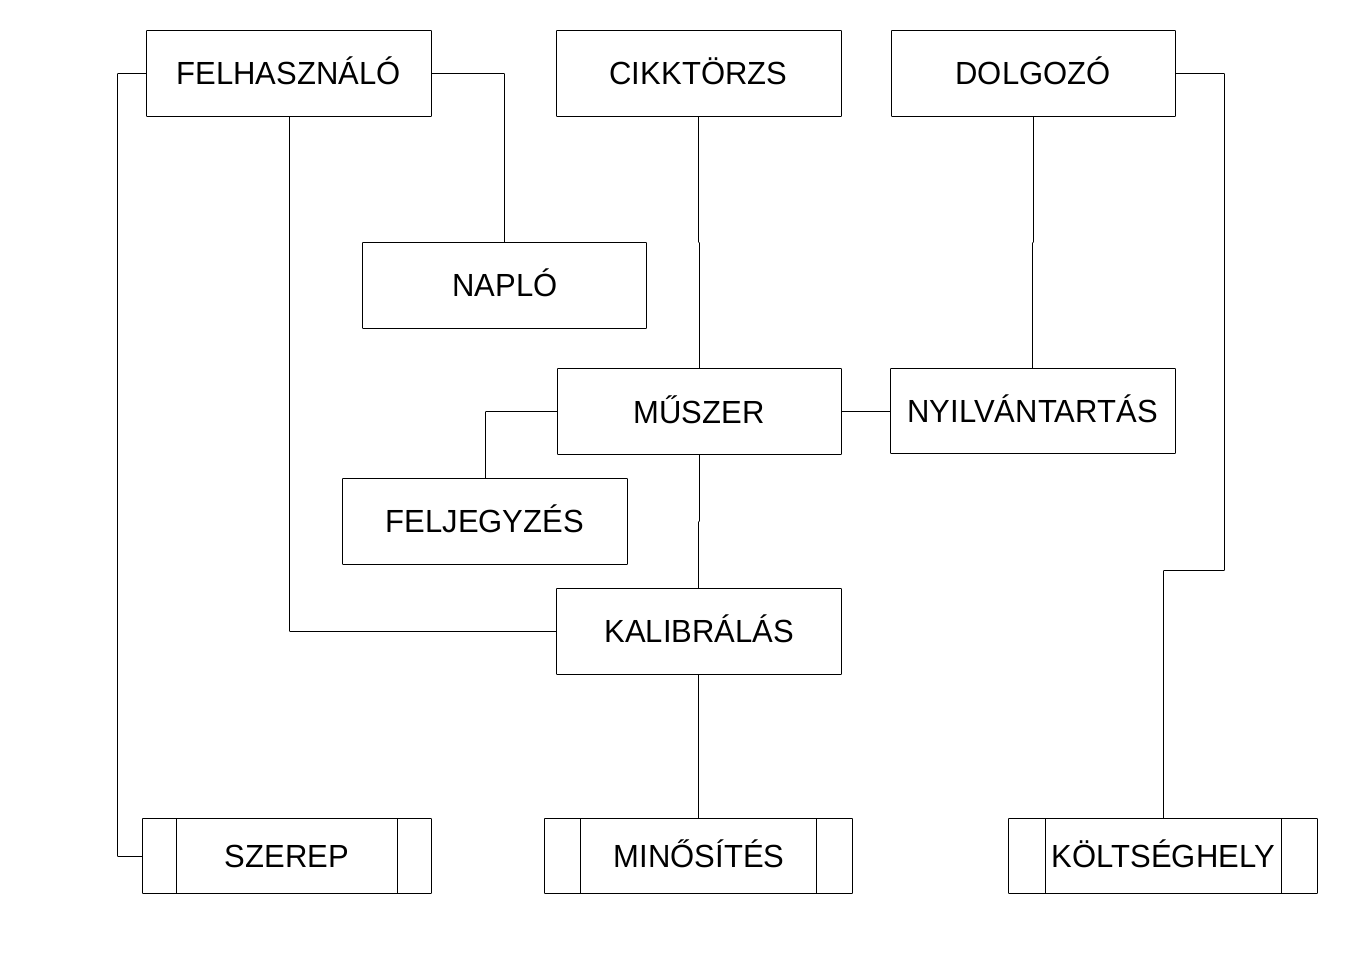
\includegraphics[width=13cm]{kepek/tablak0-kapcs0.png}
\caption{A táblák és a közöttük lévő előzetes kapcsolatok}
\end{figure}

A kapcsolatok ábrázolásánál most még foglalkozunk azzal hogy a kapcsolat 
kötelező-e, vagy opcionális, csupán jelezzük, hogy a táblák között van 
valamilyen kapcsolat. Nem jelezzük a kapcsolat fokát, ami lehet \textbf{1:1, 
1:n, m:n} sem.

\section{A táblák részletes leírása}
A táblák leírása első lépésben szöveges formában történik, az alábbi 
jelölésekkel:
\begin{itemize}
 \item \TABLA{nagybetűs} szedéssel a táblák neve szerepel: \TABLA{dolgozó}
 \item a tábla mezői zárójelek között lesznek felsorolva:\\ 
 \TABLA{DOLGOZÓ}(\PK{törzsszám}, \FK{költséghely}, név, aktív)
 \item \PK{félkövér szedéssel} a tábla kulcsát jelöljük: \PK{törzsszám}
 \item a idegen(külső) kulcsok \FK{aláhúzással} jelenek meg: 
 \FK{költséghely}
 \item félkövér és aláhúzott szöveg jelöli, ha a mező az egyik táblában kulcs 
és egy másik tábla idegen kulcsa \PK{\FK{raktárhely}} 
\item normál szedésse a tábla egyéb mezői fognak szerepelni.
\item az összetett kulcsok mezőit $+$ jel köti össze: \PK{cikkszám+sarzs}
\item abban az esetben, ha egy mező név több táblában is szerepel, a mezőt 
a tábla nevével együtt írjuk le, a tábla neve és a mező neve közé .-ot 
(pontot) teszünk: \TMEZO{KÖLTSÉGHELY}{költséghely}
\item a pillanatnyilag érdektelen részeket a \dots jelöli:
\TABLA{cikkszám}(\PK{cikkszám}, megnevezés, \dots, pontosság)
\item táblázatos megjelenítés esetén előfordul, hogy csak a fontos mezőket 
mutatjuk be. Ilyen esetben a nem mutatott mezőket ,, \dots  '' (három pont) 
jelzi. Ha a tábla alja nyitott, az azt jelzi, hogy vannak még sorok. Az 
alul zárt tábla azt jelzi, hogy minden értéket megmutattunk.
\end{itemize}

A táblák leírását célszerű azokkal kezdeni, amelyek úgynevezett 
szótár-\footnote{kulcs--érték táblák. Például országkód--országnév}, vagy
validáló\footnote{Ilyenek a kötelezően megadandó értékkészletek táblája. 
Például a minősítés: kitűnő, jó, közepes, elégséges, elégtelen} táblák.
Az ilyen táblákra jellemző, hogy ritkán változik a tartalmuk. A táblák 
tartalmazhatnak olyan tulajdonságokat, amelyekkel a felhasználói
programoknak nyújtunk segítséget, például azzal, hogy az érték
kiválasztható-e, vagy sem, az értékek rendezést valamilyen súly alapján 
végezhetik el.

\subsection{SZEREP tábla}
A \TABLA{szerep} táblában a rendszer felhasználóihoz rendelet felhasználói 
szerepek értékkészlete jelenik meg.\\

\TABLA{SZEREP}(\PK{szerep}, aktív)
\begin{table}[ht!]
\centering
\begin{tabular}[t]{|l|l|}
\hline
 \textbf{szerep}&aktív\\\hline
 \textbf{admin}&igen\\
 \textbf{kalibráló}&igen\\
 \textbf{\dots}&\dots\\
\end{tabular}
\caption{DOLGOZÓ tábla} \label{tabSZEREP}
\end{table}


\subsection{MINŐSÍTÉS tábla}
A tábla tartalmazza a műszerek minősítéséhez használható értékeket.\\

\TABLA{MINŐSÍTÉS}(\PK{minősítés}, aktív)
\begin{table}[ht!]
\centering
\begin{tabular}[t]{|l|l|}
\hline
 \textbf{minősítés}&aktív\\\hline
 \textbf{megfelelt}&igen\\
 \textbf{tájékoztató mérésre}&igen\\
 \textbf{selejt}&igen\\
 \hline
\end{tabular}
\caption{MINŐSÍTÉS tábla} \label{tabMINOSITES}
\end{table}


\subsection{KÖLTSÉGHELY tábla}
A tábla azokat a költséghelyeket tartalmazza, amelyekhez dolgozók, vagy 
műszerek rendelhetők. Egyes költséghelyek idővel megszűnnek, újak jönnek
létre.\\

\TABLA{KÖLTSÉGHELY}(\PK{költséghely}, költséghely neve, sorrend, aktív)
\begin{table}[ht!]
\centering
\begin{tabular}[t]{|l|l|l|l|}
\hline
 \textbf{költséghely}&költséghely neve&sorrend&aktív\\ \hline
 \textbf{13-421-0}&Járműlakatos művezetőség&1&igen\\
 \textbf{13-443-0}&Műszerész művezetőség&1&igen\\
 \textbf{11-210-0}&Humánügyi és bérelsz. Oszt.&9&nem\\
 \textbf{\dots}&\dots&\dots&\dots \\
\end{tabular}
\caption{KÖLTSÉGHELY tábla} \label{tabKOLTSEGHELY}
\end{table}

\subsection{FELHASZNÁLÓ tábla}
A táblában a rendszer felhasználóit tartjuk nyilván. A rendszerhez csak 
jogosult felhasználó férhet hozzá. A felhasználókról a minimális adatokat 
tartunk nyilván\\

\TABLA{felhasználó}(\PK{felhasználónév}, vezetéknév, keresztnév, 
harmadik név, titulus, jelszó, \FK{szerep}, aktív, kezdődátum, végdátum)

\begin{table}[ht!]
 \centering
 \begin{tabular}[t]{|l|l|l|l|l|l|l|l|}
  \hline
  
\textbf{felhasználónév}&vezetéknév&\dots&\FK{szerep}
&aktív&kezdődátum&végdátum\\ \hline
  \textbf{nagye}&Nagy&\dots&\FK{admin}&igen&2020.06.01&null \\
  \textbf{kissg}&Kiss&\dots&\FK{kalibráló}&igen&2020.06.01&2021.04.24\\
  \textbf{tothb}&Tóth&\dots&\FK{lekérdező}&nem&2020.06.01&2020.09.06\\
 \end{tabular}
\caption{FELHASZNÁLÓ tábla}\label{tabFEHASZNALO}
\end{table}

\subsection{DOLGOZÓ tábla}
A tábla tartalmazza azokat a dolgozókat, akik mérőeszközökkel 
rendelkeznek, vagy rendelkeztek. A dolgozókról a minimális, a rendszer 
működése szempontjából fontos adatokat tartjuk csak nyilván.\\

\TABLA{dolgozó}(\PK{törzsszám}, vezetéknév, keresztnév, harmadik név, 
\FK{költséghely}, aktív)

\begin{table}[ht!]
 \centering
 \begin{tabular}[t]{|l|l|l|l|l|}
  \hline
\textbf{törzsszám}&vezetéknév&\dots&\FK{költséghely}&aktív\\ 
\hline
  \textbf{93456}&Nagy&\dots&\FK{13-421-0}&igen \\
  \textbf{92312}&Tóth&\dots&\FK{13-443-0}&nem \\
  \textbf{95678}&Kiss&\dots&\FK{13-422-0}&igen\\
 \end{tabular}
\caption{DOLGOZÓ tábla}\label{tabDOLGOZO}
\end{table}

\subsection{CIKKTÖRZS tábla}
A táblában a SAP rendszer adatain túl olyan adatok is tárolása kerülnek, 
amelyekre a SAP rendszer nem ad lehetőséget, viszont a műszerek
szempontjából fontosak.






%
%%
%%%
%%
% 
\end{document}
